Så løser vi den originale likningen (\ref{eq:144}) numerisk for alle 4 geometriene. Og ser på plott av verdiene for potensialet $\phi_2$ på y-aksen. På x-aksen har vi de diskrete punktene. Plottet er symmetrisk fordi geometrien er symmetrisk.

\noindent
\begin{minipage}[t]{0.45\linewidth}
    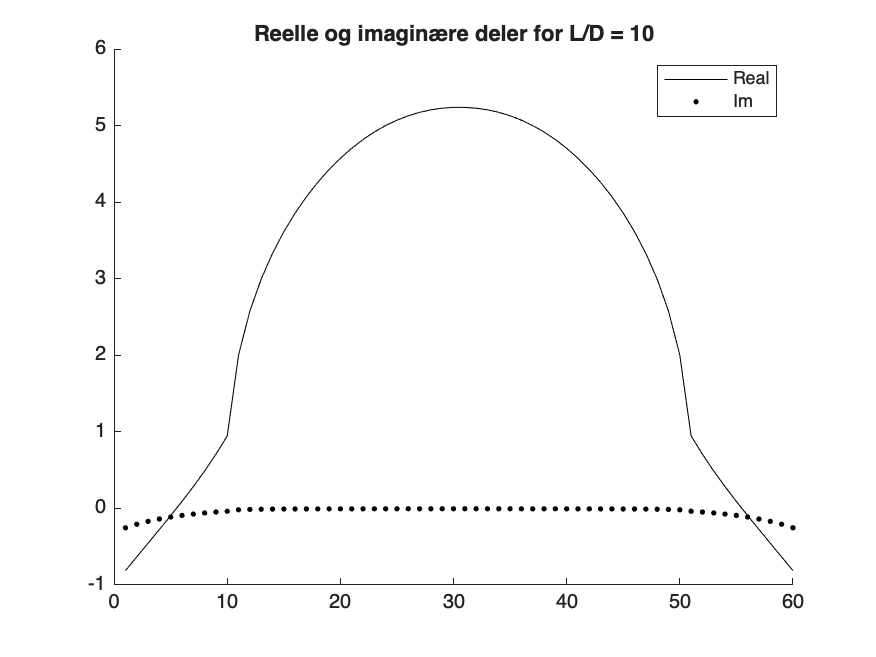
\includegraphics[width=\linewidth]{/Users/ole/Tex/MEK4420/oblig2images/plot_phi2_1.png}
    \captionof{figure}{L/D = 10}
\end{minipage}
\hspace{0.05\linewidth}
\begin{minipage}[t]{0.45\linewidth}
    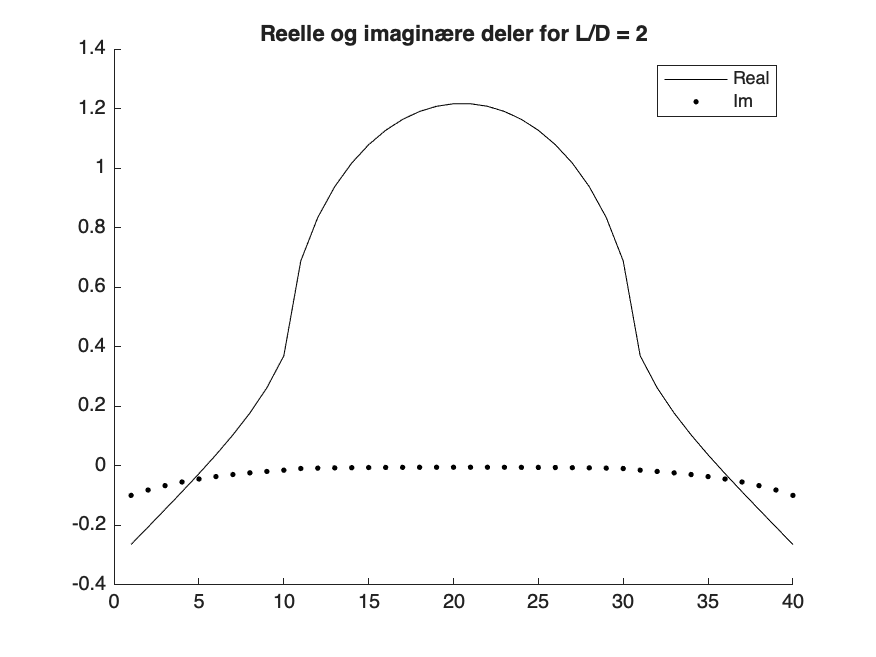
\includegraphics[width=\linewidth]{/Users/ole/Tex/MEK4420/oblig2images/plot_phi2_2.png}
    \captionof{figure}{L/D = 2}
\end{minipage}

\vspace{0.5cm} % Adds vertical space between rows

\noindent
\begin{minipage}[t]{0.45\linewidth}
    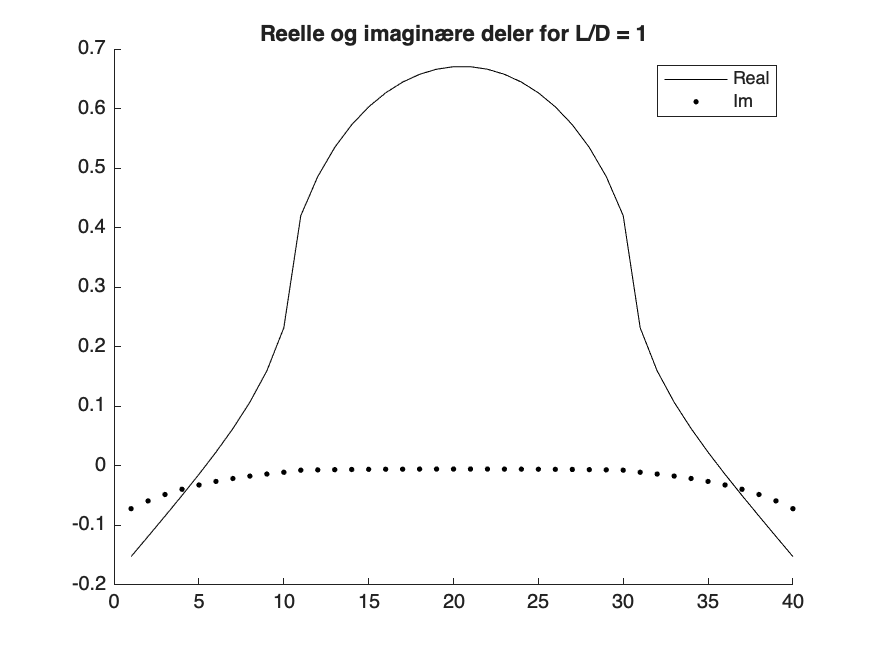
\includegraphics[width=\linewidth]{/Users/ole/Tex/MEK4420/oblig2images/plot_phi2_3.png}
    \captionof{figure}{L/D = 1}
\end{minipage}
\hspace{0.05\linewidth}
\begin{minipage}[t]{0.45\linewidth}
    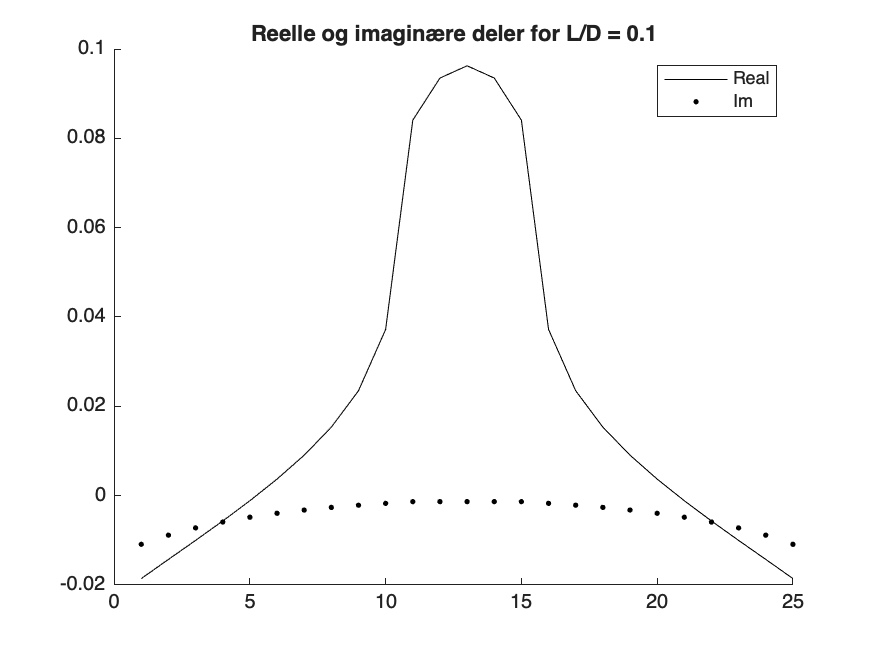
\includegraphics[width=\linewidth]{/Users/ole/Tex/MEK4420/oblig2images/plot_phi2_4.png}
    \captionof{figure}{L/D = 0.1}
\end{minipage}